\section{Parallel Bi-core Decomposition}\label{sec:par}

The sequential nature of Liu \textit{et al}'s~\cite{Liu2020Efficient} bi-core decomposition (Algorithm \ref{alg-seq}) limits its practical applicability to large graphs. While Liu \textit{et al.}~\cite{Liu2020Efficient} provides a parallel version of their algorithm, their parallel algorithm only parallelizes between rounds of peeling (subroutines \algname{peel-fix-$\alpha$} and \algname{peel-fix-$\beta$}), and does not parallelize the peeling process itself. As a result, it has a high span of $\BigO{m}$. We present in this section a parallel bi-core decomposition algorithm using the same computation-sharing technique developed by Liu \textit{et al}~\cite{Liu2020Efficient}. We prove that our algorithm is work-efficient and has span $\BigO{\rho \log(n)}$ \textit{w.h.p.}, where \emph{$\rho$} is the peeling complexity, which we define as follows.

\begin{definition}\label{def:peeling-complex}
The bi-core peeling complexity $\rho$ is the maximum number of rounds needed to empty the graph by any call of \algname{par-peel-fix-$\alpha$} or \algname{par-peel-fix-$\beta$}, where in each round of peeling, the set of vertices with the minimum induced degree is removed from the graph 
\end{definition}

It is worth remarking that the bi-core peeling complexity $\rho$ cannot be bounded by $\BigO{\rho_k}$ where $\rho_k$ is the $k$-core peeling complexity introduced by Dhulipala \textit{et al.}~\cite{DhBlSh18}.

Our algorithm is based on a peeling paradigm. For \algname{par-peel-fix-$\beta$} given a fixed $\beta'$, in each round, we remove all vertices $u$ with the lowest induced degree concurrently. In other words, we peel all vertices $u$ with $\deg(u)\le \alpha$ for the current $\alpha$. 
In order to efficiently peel these vertices concurrently, we must update the degrees of the neighbors of the peeled vertices in parallel, using an approach that we describe in Section \ref{sec:par-decomp}.
Additionally, to reduce the span of the sequential search used in Algorithm \ref{alg-seq}, we use a parallel exponential search technique to find the next set of vertices with minimum degree; we discuss this in Section \ref{sec:par-buckets}. 

\subsection{Parallel Bucketing and Exponential Search}
\label{sec:par-buckets}
To achieve polylogarithmic span while maintaining work-efficiency, we use an efficient parallel bucketing structure to store the subset of vertices to be peeled in each round. Dhulipala \textit{et al.} introduced this parallel bucketing structure and applied it to their parallel $k$-core decomposition algorithm \cite{DhBlSh17}. 
The data structure consists of an array of buckets, where the indices represent vertex degrees.
Each bucket stores all vertices with current degree corresponding to its index. It supports two types of operations. \algname{update-vertices} allows batch update of vertices' degrees. It moves those vertices to new buckets corresponding to their new degrees in parallel \cite{DhBlSh17}. On the other hand, \algname{next-bucket}, given a degree value $k$, searches for the next subset of vertices with lowest induced degree $\ge k$. We introduce a parallel exponential search to complete this in logarithmic span. We provide its pseudocode in Algorithm \ref{alg-bucket}. 

\begin{algorithm}[t!]
 \footnotesize
\caption{Parallel Exponential Search}
 \begin{algorithmic}[1]
 
 \Procedure{Has-Min-Deg}{$\text{buckets}$} \Comment{check if the given slice of array of buckets contain a nonempty bucket}
 \State $\text{hasMinDeg}\leftarrow \textit{false}$ \Comment{$\text{hasMinDeg}$ records whether the interval contain the next nonempty bucket}
 \ParFor{$i=0$ to $|\text{buckets}|$}
 \If{$\text{buckets}[i]$ exists}
 \State \algname{atomic-compare-and-swap}($\text{hasMinDeg}, \textit{false}, \textit{true}$) 
 \EndIf
 \EndParFor
 \State \Return $\text{hasMinDeg}$ 
 \EndProcedure
 
 \Procedure{Next-Bucket}{$\text{buckets}$, $k$} \Comment{find and return the next nonempty bucket and its corresponding degree}
 \State $i\leftarrow 1$ \Comment{$i$ is doubled in each iteration of the while loop. In each iteration, we search interval $(\frac{i}{2},i]$ for the next nonempty bucket}
 \While{\algname{Has-Min-Deg}($\text{buckets}[k+\frac{i}{2}+1\ \text{to}\ k+i]$)$=\textit{false}$} \label{alg-next-bucket:start-while}
 \State $i\leftarrow 2i$
 \EndWhile \label{alg-next-bucket:end-while}
 \State $\text{minDeg}\leftarrow\ $ \algname{reduce-min}(\text{buckets}$[k+\frac{i}{2}+1\ \text{to}\ k+i]$)
 \State \Return $\text{buckets}[\text{minDeg}], 
 \text{minDeg}$ \Comment{Return next min deg}
 \EndProcedure
 
 \end{algorithmic}
 \label{alg-bucket}
\end{algorithm}

\algname{next-bucket} finds and returns the next nonempty bucket with degree $\ge k$. First, we initialize $i$ to $1$. Then, in each iteration of the while loop on Lines \ref{alg-next-bucket:start-while}--\ref{alg-next-bucket:end-while} of Algorithm \ref{alg-bucket}, we determine if the interval $(k+\frac{i}{2},k+i]$ contains the next nonempty bucket. Then, we double $i$ and repeat until the next nonempty bucket is found. For instance,  we start the search from the interval $(k,k+1]$. The \algname{has-min-deg} subroutine called on Line \ref{alg-next-bucket:start-while} checks in parallel whether the next minimum degree vertex exist in the given interval. If it does not exist in this interval, we proceed to interval $(k+1,k+2]$, and then to $(k+2,k+4],(k + 2^i, k + 2^{i+1})$ for each $i$ until a nonempty bucket is found. 

On Line 11, we perform a parallel \algname{reduce-min} on the sequence of the indices of nonempty buckets to obtain the next minimum degree with nonempty bucket. On Line 12, we return the next nonempty bucket.

\myparagraph{Analysis}

First, let $n$ be the number of vertices stored in the bucketing structure. 

Given $p$ calls to \algname{update-vertices} updating a total of $q$ vertices (a repeating vertex is counted repeatedly), \algname{update-vertices} achieves an overall work complexity of $\BigO{q}$ and span complexity of $\BigO{p\log(n)}$ \cite{DhBlSh17}.

We perform $p$ calls to \algname{next-bucket} with the condition that the degree value $k$ passed in at the $i^\text{th}$ call equals the return value of the $(i-1)^\text{th}$ call. In other words, we find the next nonempty bucket starting from the previous nonempty bucket. Given the condition, over all $p$ calls to subroutine \algname{next-bucket}, we now show that it achieves an overall work complexity of $\BigO{n}$ and span complexity of $\BigO{p\log(n)}$.

Assume \algname{next-bucket} is called with current degree value $k$ and that the next minimum degree is $k+h$. Then, notice that \algname{next-bucket} searches at most $2h$ elements before terminating and returning $k + h$ as the next minimum degree. If it searches only $h$ elements ahead, the algorithm has an overall work upperbounded by $\BigO{\text{dmax}_v}=\BigO{n}$. Since it searches only $2p$ ahead, its work is bounded by $\BigO{2n}=\BigO{n}$ as well.

Next, we show that the subroutine \algname{next-bucket} has a span of $\BigO{p\log(n)}$. Assume, as previously, that the current degree is $k$ and the next degree is $k+h$. Note that \algname{next-bucket} takes at most $\log(h)$ iterations of its while loop on Line 9 of Algorithm \ref{alg-bucket} to find the next minimum degree $k+h$. To loosen the bound, $\log(h)=\BigO{\log(n)}$. Therefore, the overall span of $p$ calls to \algname{next-bucket} is $\BigO{p \log(n)}$. An assumption we make in this derivation is that subroutine \algname{has-min-deg} as used on Line 9 has span $\BigO{1}$. This is true because at most one \algname{atomic-compare-and-swap} operation can be successfully executed for a given interval. Additionally, note that \algname{reduce-min} on Line 11 of Algorithm \ref{alg-bucket} has span $\BigO{\log(n)}$; it is executed only once for each call of \algname{next-bucket}, thus totaling a span of $\BigO{p\log(n)}$ as well.

% \subsection{Parallel Peeling}\label{sec:par-peel}
% \begin{algorithm}[t!]
%  \footnotesize
% \caption{Parallel Peeling}
%  \begin{algorithmic}[1]
% \Procedure{Par-Del-Update}{$G$, $X_\text{del}$} 
%  \State $Y_\text{update}\leftarrow \emptyset$
%  \State $\text{degs}\leftarrow$ array storing the corresponding degree of each vertex $x\in X_\text{del}$ 
%  \State $\text{offsets}\leftarrow$ \algname{prefix-sum}($\text{degs}$)
%  \ParFor{\textbf{all} $i,x$ in $X_\text{del}$}
%  \State remove $x$ from $G$
%  \ParFor{\textbf{all} $y$ in $N(x)$}
%  \State $\text{offset}\leftarrow \text{offsets}$[$i$]$+j$ \Comment{Obtain the location in $Y_\text{update}$ to store $y$ at. $j$ is the index of $y$ in $N(x)$}
%  \State $Y_\text{update}$[$\text{offset}$] $\leftarrow y$ \Comment{Record $y$ for degree update}
%  \EndParFor
%  \EndParFor
%  \State $Y_\text{hist} \leftarrow $ \algname{histogram}($Y_\text{update}$) \Comment{Count occurrences of vertices}
%  \ParFor{\textbf{all} $y,\text{count}$ in $Y_\text{hist}$}
%  \State $\deg(y) \leftarrow \deg(y)-\text{count}$ 
%  \EndParFor
%  \State \Return $Y_\text{update}$
%  \EndProcedure
%   \end{algorithmic}
%  \label{alg-peel}
% \end{algorithm}

% \jessica{you haven't introduced Algorithm \ref{alg-par} yet! Don't reference pseudocode for parts that you haven't talked about in detail yet. I also don't understand why this has to be separated from what you talk about in 5.3, since it doesn't make much sense as a standalone, without talking about 5.3 first. I would just merge this with Algorithm \ref{alg-par}, and talk about both like you do sequentially. This is relatively short anyways}
% At the crux of \algname{par-peel-fix-$\alpha$} and \algname{par-peel-fix-$\beta$} of Algorithm \ref{alg-par} is the \algname{par-del-update} operation which takes as input a generic subset of vertices $X_\text{del}$ and then peels all its vertices in parallel. On Lines 7--9, we iterate through all neighbors $y$ of $X_\text{del}$ and store them in an array $Y_\text{update}$. We filter out already deleted vertices on Line 10 using \algname{filter}. On Line 11, \algname{histogram} returns a sequence of pairs $(y,\text{count})$. For every $y$, $\text{count}$ is the number of its occurrences in $Y_\text{update}$. On Lines 12--13, we iterate through each $y$ and decrease its degree by its corresponding $\text{count}$. 

% Since many threads may be updating the degree of the same vertex, our parallel aggregation approach is necessary to maintain low theoretical span.

% \myparagraph{Analysis}
% In each complete $\beta$-core peeling \jessica{I don't think this is clear; the reader doesn't necessarily know what you mean by "complete" peeling; also, I seem to recall in the sequential setting that you peel on the $\alpha$ side by default in your explanations -- this should be consistent? Another note about notation -- I've been removing places where you say "$\alpha$-core peeling" or "$\beta$-core peeling," because it's imprecise and the peeling process for k-core can be confused with it. It should be about peeling an $(\alpha, \beta)$-core, not $\alpha$-core or $\beta$-core.}, each vertex is peeled exactly once. Since we traverse the neighbor of each vertex in \algname{par-del-update} once, the total work given by \algname{par-del-update} in one complete $\beta$-core peeling \jessica{fix} is $\BigO{\sum_{x\in {V\text{ or }U}} \deg(i)}=\BigO{m}$ \jessica{should be $\text{deg}(x)$?}. This matches the best theoretical time complexity for the sequential algorithm (Algorithm \ref{alg-seq}) \jessica{this is confusing because the alg you're referencing is the full peeling alg, and this is just some subroutine -- I think it'll be clearer if you combine this with the next subsection}. Thus, \algname{par-del-update} is work-efficient. 

% The span of \algname{par-del-update} is bounded by $\BigO{\log(n)}$. Lines 5--9 have span $\BigO{1}$ due to arbitrary forking. \algname{prefix-sum}, \algname{filter}, \algname{histogram} all have span bounded by $\BigO{\log(n)}$. Therefore, the overall span is $\BigO{\log(n)}$.

\subsection{Parallel Bi-core Decomposition}
\label{sec:par-decomp}
\begin{algorithm}[t!]
 \footnotesize
\caption{Parallel Bi-core Decomposition}
 \begin{algorithmic}[1]
 
 \Procedure{par-bi-core}{$G$}
 \ParFor{$\alpha'=1$ to $\delta$}
 \State \Call{Par-Peel-Fix-$\alpha$}{$G$, $\alpha'$}
 \EndParFor
 \ParFor{$\beta'=1$ to $\delta$}
 \State \Call{Par-Peel-Fix-$\beta$}{$G$, $\beta'$}
 \EndParFor
 \EndProcedure

\Procedure{Par-Del-Update}{$G$, $X_\text{del}$} 
 \State $Y_\text{update}\leftarrow \emptyset$
 \State $\text{degs}\leftarrow$ array storing the corresponding degree of each vertex $x\in X_\text{del}$ 
 \State $\text{offsets}\leftarrow$ \algname{prefix-sum}($\text{degs}$)
 \ParFor{\textbf{all} $i,x$ in $X_\text{del}$}
 \State remove $x$ from $G$
 \ParFor{\textbf{all} $y$ in $N(x)$}
 \State $\text{offset}\leftarrow \text{offsets}$[$i$]$+j$ \Comment{Obtain the location in $Y_\text{update}$ to store $y$ at. $j$ is the index of $y$ in $N(x)$}
 \State $Y_\text{update}$[$\text{offset}$] $\leftarrow y$ \Comment{Record $y$ for degree update}
 \EndParFor
 \EndParFor
 \State $Y_\text{hist} \leftarrow $ \algname{histogram}($Y_\text{update}$) \Comment{Count occurrences of vertices}
 \ParFor{\textbf{all} $y,\text{count}$ in $Y_\text{hist}$}
 \State $\deg(y) \leftarrow \deg(y)-\text{count}$ 
 \EndParFor
 \State \Return $Y_\text{update}$
 \EndProcedure

\Procedure{Par-Peel-Fix-$\beta$}{$G$, $\beta'$}
 \State \Call{par-del-update}{$G$, $\{ v | \deg(v)<\beta' \}$} \Comment{Remove all vertices in $V$ with degree $< \beta'$}
 \State Store vertices in $U$ into $\text{buckets}$ \Comment{Construct bucketing structure from vertices in $U$ based on their degrees}
 \While{$\text{buckets}\ne \emptyset$}
     \State $U_\text{del},\alpha \leftarrow$ \algname{next-bucket}($\text{buckets}$, $\alpha$) \Comment{Extract the next set of vertices with minimum degree}
     \ParFor{\textbf{all} $u$ in $U_\text{del}$}
     \ParFor{$i=1$ to $\alpha$}
        \State $\beta_{\max i}(u) \leftarrow \max(\beta_{\max i}(u),\beta')$ \Comment{Update $\beta_{\max i}(u)$}
     \EndParFor
     \EndParFor
     \State $V_\text{update}\leftarrow$ \algname{par-del-update}($G$, $U_\text{del}$) \Comment{Peel $U$ up to $\alpha$}\label{peelu}
     \State $V_\text{del}\leftarrow$ \Call{filter}{$V_\text{update}$, $\deg(v)< \beta'$}
     \ParFor{\textbf{all} $v$ in $V_\text{del}$}
     \State $\alpha_{\max \beta'}(v)\leftarrow \max(\alpha_{\max \beta'}(v), \alpha)$ \Comment{Update $\alpha_{\max \beta'}(v)$}\label{updatealpha}
     \EndParFor
     \State $U_\text{update} \leftarrow$ \algname{par-del-update}($G$, $V_\text{del}$) \Comment{Remove peeled $v$}\label{removev}
    \State $\text{buckets}$.\algname{update-vertices}($U_\text{update}$) \Comment{Update vertices with changed degrees in the bucketing structure}
 \EndWhile
 \EndProcedure

\Procedure{Par-Peel-Fix-$\alpha$}{G, $\alpha'$}
 \State symmetric to \algname{Par-Peel-Fix-$\beta$}
 \EndProcedure
 \end{algorithmic}
 \label{alg-par}
\end{algorithm}

The parallel bi-core decomposition algorithm shares a similar structure to Algorithm \ref{alg-seq}. Instead of removing vertices with minimum induced degree sequentially, we delete all vertices with the same minimum induced degree in parallel. Further, to achieve optimal span, we replace the linear search used in Algorithm \ref{alg-seq} to find the next lowest degree vertex with Algorithm \ref{alg-bucket} to find the next bucket of vertices with lowest induced degree.   

The pseudocode is given in Algorithm \ref{alg-par} and we now discuss it in more detail. 

First we discuss the subroutine \algname{par-del-update}. Subroutine \algname{par-del-update} takes as input a generic subset of vertices $X_\text{del}$ and then peels all these vertices in parallel. On Lines 7--14, we construct an array $Y_\text{update}$ that stores all neighbors $y$ of $X_\text{del}$. Note that if $y$ is incident to multiple vertices in $X_\text{del}$, it appears the same number of times in $Y_\text{update}$. This array is constructed in parallel by first building the array $\text{offsets}$ as the \algname{prefix-sum} of $\text{degs}$ on Line 9. $\text{offsets}[i]$ records the total number of neighbors of vertices $[1,2,\cdots,i-1]$ in $X_\text{del}$. Therefore, $\text{offsets}[i]+j$ gives the index location to store the $j^\text{th}$ neighbor of the $i^\text{th}$ vertex in $X_\text{del}$, which is used on Lines 13-14 to store neighbor $y$ into its place in $Y_\text{update}$. On Line 15, \algname{histogram} returns a sequence of pairs $(y,\text{count})$. For every $y$, $\text{count}$ is the number of its occurrences in $Y_\text{update}$. On Lines 12--13, we iterate through each $y$ and decrease its degree by its corresponding $\text{count}$. Note that on Line 11, it is unnecessary to remove $x$ from $G$. We can simply maintain an array that tracks whether each vertex is removed and ignore vertices marked as removed in our traversals. 

Since many threads may be updating the degree of the same vertex, our parallel aggregation approach is necessary to maintain low theoretical span.

Now, we discuss the main algorithm. 
On Line 20 in \algname{par-peel-fix-$\beta$}, we peel off all $v\in V$ with degree less than $\beta'$ using the subroutine \algname{par-del-update}. On Line 21, we construct a bucket representation of $U$, buckets, as discussed by Dhulipala \textit{et al.}~\cite{DhBlSh17} and as described in Section \ref{sec:par-buckets}. We call \algname{next-bucket} on $\text{buckets}$ on Line 23 to obtain the next nonempty bucket, which we store into $U_\text{del}$. We also update the $\alpha$ value appropriately; importantly, $U_\text{del}$ records all $u$ with induced degree $\deg(u)\le \beta$. Note that for all $u\in U_\text{del}$, $u\in (\alpha',\beta)$-core but $u\not\in (\alpha',\beta+1)$-core. On Lines 24--26, we in parallel update the $\beta_{\max \alpha'}$ values. Note that Line 26 does not incur race conditions if we keep a copy of $\beta_{\max \alpha}$ and similarly $\alpha_{\max \beta}$ for each thread. 
On Line 27, we peel off all vertices in the current bucket, $U_\text{del}$. Lines 29--30 updates $\alpha_{\max \beta'}$ values in the same way as in Algorithm \ref{alg-seq}. Then, Line 31 calls \algname{par-del-update} to peel off all vertices stored in $V_\text{del}$. Finally, on Line 32, we update the degrees of vertices in $U_\text{update}$, which consist of all vertices $u\in U$ whose degree is affected by peeling off $V_\text{del}$; \algname{update-vertex} moves $y\in U_\text{update}$ to new buckets corresponding to their new degrees. Note that a minor detail we exclude here is that some vertices in $U_\text{update}$ could take on a degree $< \alpha$. We simply set their degree to $\alpha$, so they are peeled together in the next round of peeling.

\algname{par-peel-fix-$\alpha$} is symmetric to \algname{par-peel-fix-$\beta$}, with all $u,v$ and $\alpha,\beta$ flipped.

\myparagraph{Analysis}
\algname{par-peel-fix-$\beta$} has work complexity $\BigO{m}$. First note that \algname{next-bucket}, and \algname{update-vertices}~\cite{DhBlSh17} all have overall work across all iterations of the while loop bounded by $\BigO{m}$ as discussed in Section \ref{sec:par-buckets}.

Over all invocations of subroutine \algname{par-del-update}, each vertex is peeled exactly once. Since we traverse the neighbor of each vertex in \algname{par-del-update} once, the total work given by \algname{par-del-update} in one call of \algname{par-peel-fix-$\beta$} is $\BigO{\sum_{x\in {V\text{ or }U}} \deg(x)}=\BigO{m}$.

The work of updating the $\beta_{\max \alpha}$ and $\alpha_{\max \beta}$ values in Algorithm \ref{alg-par} is the same as the sequential updates performed in Algorithm \ref{alg-seq}, totaling $\BigO{m}$. \algname{filter}, over all invocations, also total $\BigO{m}$ work. Therefore, \algname{par-peel-fix-$\beta$} has work complexity $\BigO{m}$. Thus, procedure \algname{par-bi-core} has overall work complexity $\BigO{\delta m}$ or more loosely $\BigO{m^\frac{3}{2}}$.

Now we analyze the span complexity. 
First note that \algname{par-del-update} has span $\BigO{\log(n)}$ \textit{w.h.p.}; this is because \algname{prefix-sum} and \algname{histogram} both have span upperbounded by $\BigO{\log(n)}$ \textit{w.h.p.}.  
Each iteration of the while loop on Line 22 has span $\BigO{\log(n)}$ \textit{w.h.p.} because \algname{filter}, \algname{par-del-update}, \algname{update-vertices}~\cite{DhBlSh17}, and \algname{next-bucket} all have span bounded by $\BigO{\log(n)}$ \textit{w.h.p.}. The rounds of iterations of the while loop is bounded by $\BigO{\rho}$. The span is therefore $\BigO{\rho\log(n)}$ \textit{w.h.p.}. Overall, \algname{par-bi-core} has span $\BigO{\rho \log(n)}$ \textit{w.h.p.}.

\subsection{P-completeness}

The span of our algorithm is not polylogarithmic. However, this is to be expected as the problem of bi-core decomposition is P-complete, which we prove here. We prove the P-completeness of the decision version of the bi-core decomposition problem. The decision problem is: given values $\alpha, \beta$ and a simple bipartite graph, decide if $(\alpha, \beta)$-core is nonempty in the graph. This is a generalization of the $k$-core decision problem on a bipartite graph: given value $k$, decide if $(k,k)$-core exists. We show the P-completeness of bi-core decision problem using a reduction from the $k$-core decision problem. 

\begin{theorem}
The $(\alpha,\beta)$-core decomposition problem is P-complete if and only if $\alpha \ge 3$ or $\beta \ge 3$. Otherwise, if $\alpha \leq 2$ and $\beta \leq 2$, it is in NC.
\end{theorem}

\myparagraph{When $\alpha \leq 2$ and $\beta \leq 2$}
For $\alpha= 2$ or $\beta= 2$, the $(2,2)$-core decomposition problem is equivalent to the $k$-core decomposition problem on the bipartite graph with $k=2$, which has an NC solution \cite{Anderson84}.

If $\alpha=1$, then the $(1,\beta)$-core decomposition problem is equivalent to finding all vertices $x\in V$ such that $\deg(x)\ge \beta$ as well as its neighbors in partition $U$. Similarly, we can solve $(\alpha,1)$-core decomposition for some arbitrary $\alpha$ with $\BigO{1}$ span.

\myparagraph{When $\alpha\ge 3$ and $\beta \ge 3$}
We perform the reduction from the $k$-core decision problem in a general graph $G$ by constructing $G'$ such that $G'$ is bipartite and the $k$-core decision problem on $G$ is equivalent to the $(k,k)$-core decision problem on $G'$. 

Let $G'$ consist of two partitions $U, V$ where each partition is a copy of all vertices of $G$. In other words, a vertex $x\in G$ is copied to $x_u$ and $x_v$ in $G'$. Now, we connect an edge $(x_u, y_v)$ in $G'$ if $(x,y)$ is an edge in $G$. 

Now, we show that for any value $k$, $k$-core is nonempty in $G$ if and only if $(k,k)$-core is nonempty in $G'$. If the $k$-core of $G$ is nonempty and comprises a vertex subset $W$, then for $w\in W$, $\deg(w)\ge k$, or there exists $\ge k$ edges of the form $(w, p)$, where $p\in W$. Now consider $W' = W_V\bigcup W_U$ in $G$. Given that $W_U, W_V$ are copies of $W$, and each $w\in W$ has $\ge k$ edges of the form $(w, p)$, we know each $w_U\in W_U$ is incident to $\ge k$ edges of the form $(w_U, p_V)$. Similarly for each $w_V\in W_V$. Therefore, $W'$ forms a $(k,k)$-core on the bipartite graph and so the $(k,k)$-core is nonempty in $G'$. 

Reversely, if the $(k,k)$-core in $G'$ is nonempty, we show that the $k$-core in $G$ is nonempty. Due to the symmetry of $U,V$ partitions, if $w_U\in (k,k)$-core, then $w_V\in (k,k)$-core. Therefore, if the $(k,k)$-core of $G'$ is $W'$, then $W' = W_U \bigcup W_V$ and $W_U, W_V$ are mirror images of each other. Let $W$ be the vertex subset in $G$ that corresponds to $W_U, W_V$. We show that it is a $k$-core in $G$. For each vertex $w_U$ incident to edges of the form $(w_U, p_V)$ where $p_V\in W_V$, its corresponding vertex $w$ in $W$ is incident to the corresponding edges of the form $(w,p)$ and $p\in W$ because $p_V\in W_V$. Since $\deg(w_U)\ge k$ for each $w_U\in W_U$, $\deg(w)\ge k$ for each $w\in W$. Therefore, $W$ forms a $k$-core of graph $G$ and so the $k$-core of graph $G$ is nonempty. 

Given the correspondence between the $k$-core decision problem on graph $G$ with the $(k,k)$-core decision problem on graph $G'$, we have obtained an NC reduction from the $k$-core problem to the bi-core problem since constructing $G'$ takes work $\BigO{m}$ and span $\BigO{1}$. Therefore, given that $k$-core decomposition is P-complete for $k\ge 3$, we know that bi-core decomposition is P-complete for $\alpha\ge 3, \beta\ge 3$.

\myparagraph{When one of $\alpha$, $\beta$ $=2$}
For the case where $\alpha=2$ and $\beta$ is some arbitrary value $\ge 3$ (the reverse of this is symmetric and thus not shown). We show that deciding whether $(2,\beta)$-core is nonempty has a reduction from the $k$-core equivalent with $k=\beta$. Consider an arbitrary simple graph and the $k$-core problem on this graph. We create a middle-vertex for each edge in the graph. Putting these middle-vertices into the $U$ partition and the original vertices into the $V$ partition, we can create in $\BigO{1}$ span a bipartite graph where all vertices in $U$ has a degree of $2$. Now, deciding if $(2,\beta)$-core nonempty is equivalent to deciding if the $k$-core of the original graph is nonemtpy, where $k=\beta$, because each wedge in the bipartite graph corresponds to an edge in the original graph. Given this reduction, we know the problem of bi-core decomposition is P-complete if the core $(\alpha,\beta)$ is of the form $(2,\beta)$ with $\beta\ge 3$ or $(\alpha,2)$ with $\alpha\ge 3$.

Thus, we have proven that the bi-core decomposition problem is in NC if and only if $\alpha= 1$ or $\beta= 1$ or $\alpha,\beta = 2$. Otherwise, it is P-complete, meaning that it is most likely impossible to obtain an algorithm with polylogarithmic span.


\subsection{Peeling Space Pruning Optimization}\label{sec:optim}
In this section, we introduce a peeling space pruning optimization to our algorithm. This optimization is also applicable to the sequential bi-core decomposition algorithm in Algorithm \ref{alg-seq}. The baseline algorithm introduced by Liu \textit{et al.}~\cite{Liu2020Efficient} performs a complete peeling from $\alpha=1$ to $\alpha=\text{dmax}_u$ for each $1\le \beta'\le \delta$. Then, it performs a complete peeling from $\beta=1$ to $\beta=\text{dmax}_v$ for each $1\le \alpha'\le \delta$.
We observe that, in the process of peeling, all $(\alpha,\beta)$-cores with $1\le\alpha\le \delta$ and $1\le\beta\le\delta$ are peeled twice, once when we perform peeling along increasing $\alpha$ values for different $\beta'$ and another time when we perform peeling along increasing $\beta$ values for different $\alpha'$. 

To avoid repetition, we can modify Algorithm \ref{alg-par} such that each \algname{par-peel-fix-$\alpha$}($G,\alpha'$) starts peeling along $\beta$ values from the $(\alpha',\alpha')$-core instead of from $(\alpha',1)$-core. In other words, the algorithm starts iteratively increasing $\beta$ value from $\alpha'$ to $\text{dmax}_v$ and removing vertices no longer within the current $(\alpha',\beta)$-core at the same time. Notably, we confine $\beta$ to $\alpha'\le\beta\le\text{dmax}_v$ as opposed to $1\le\beta\le\text{dmax}_v$ as used in Algorithms \ref{alg-seq} and \ref{alg-par}.

We illustrate this optimization with an example. Consider a graph and its peeling space visualization as shown in Figure \ref{fig:peel}.

\begin{figure}%
    \centering
    \subfloat[\centering Example Graph]{{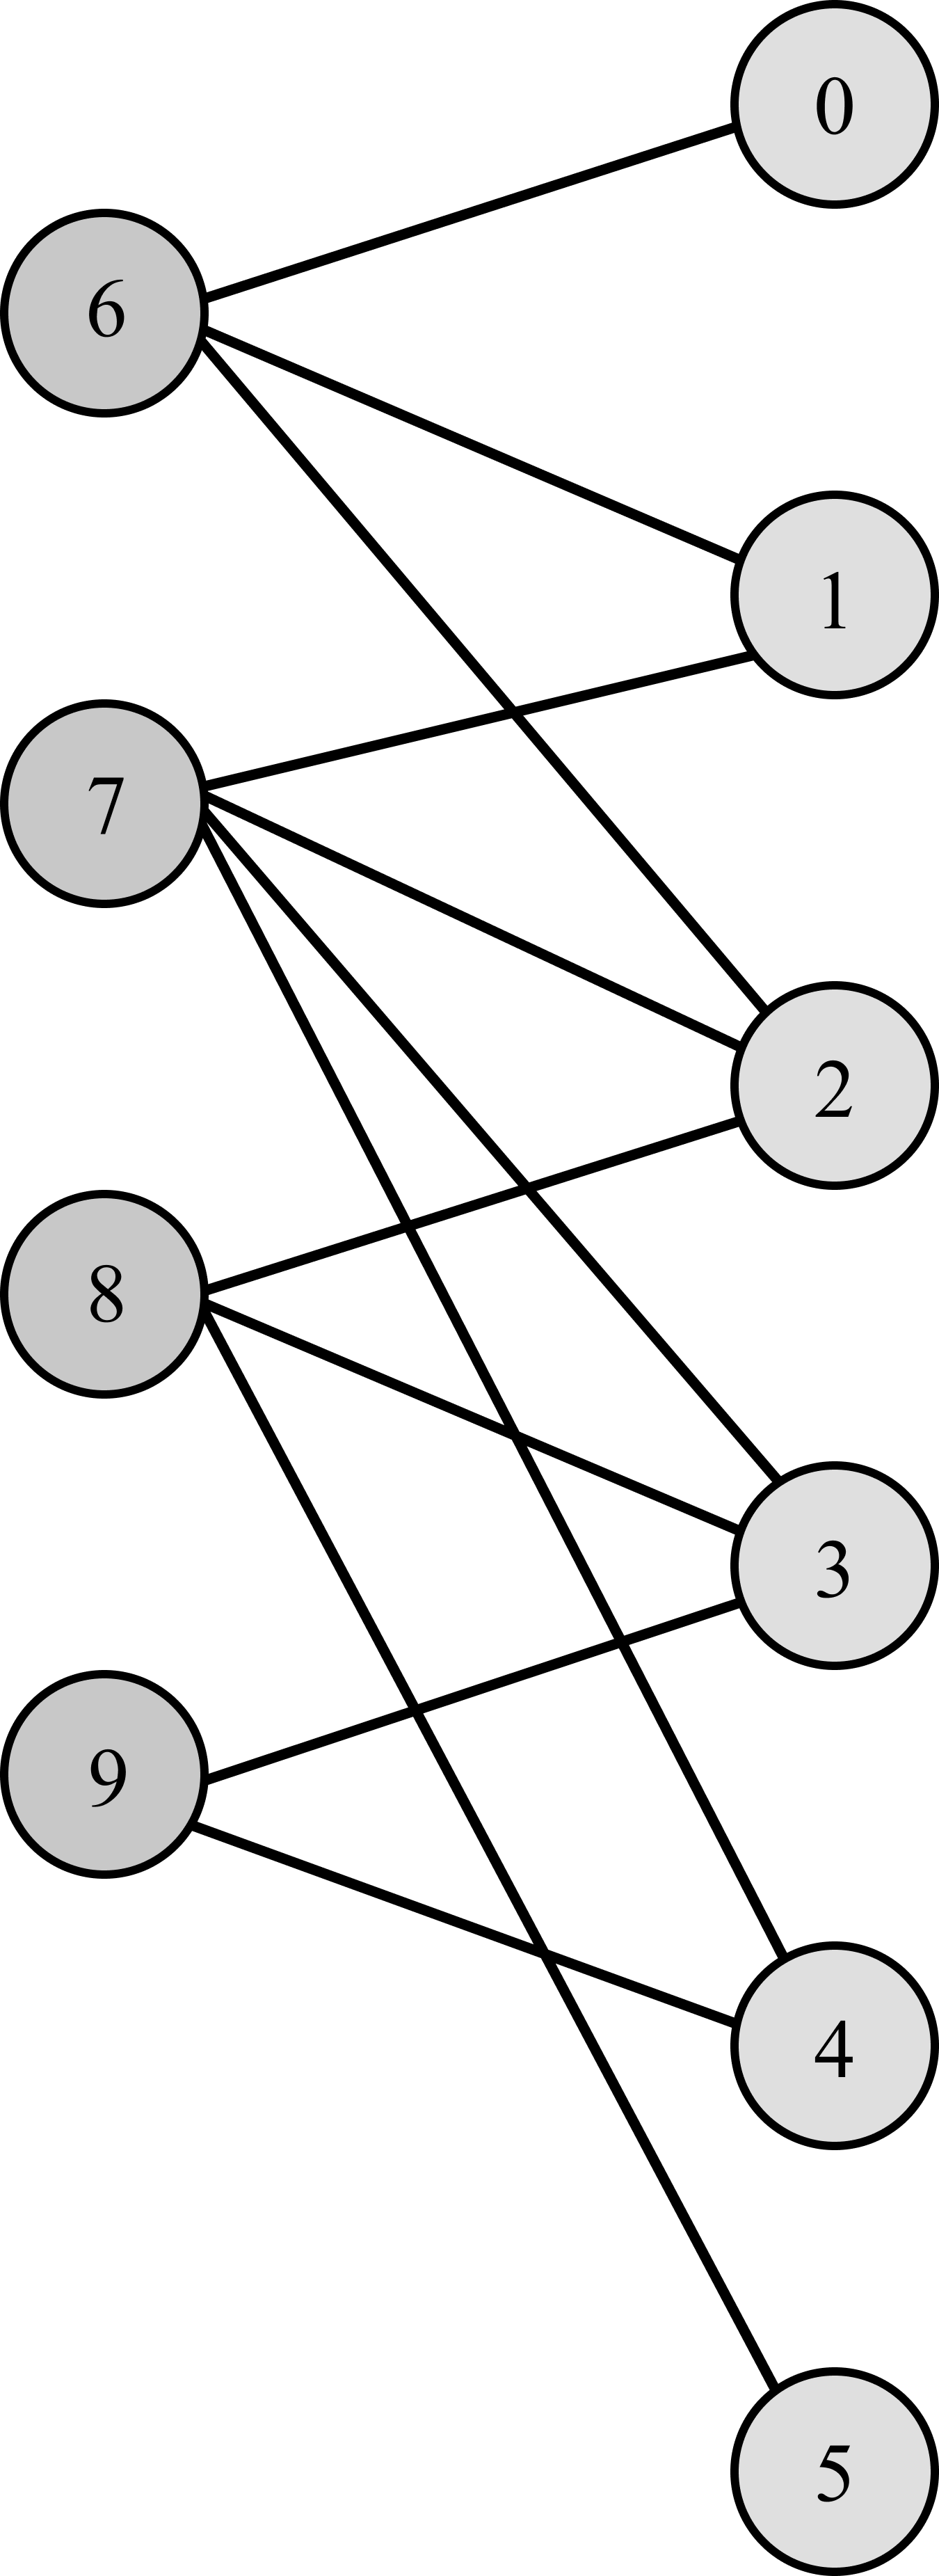
\includegraphics[height=7cm]{figures/bipartite.png} }}%
    \qquad
    \subfloat[\centering Example Peeling Space ]{{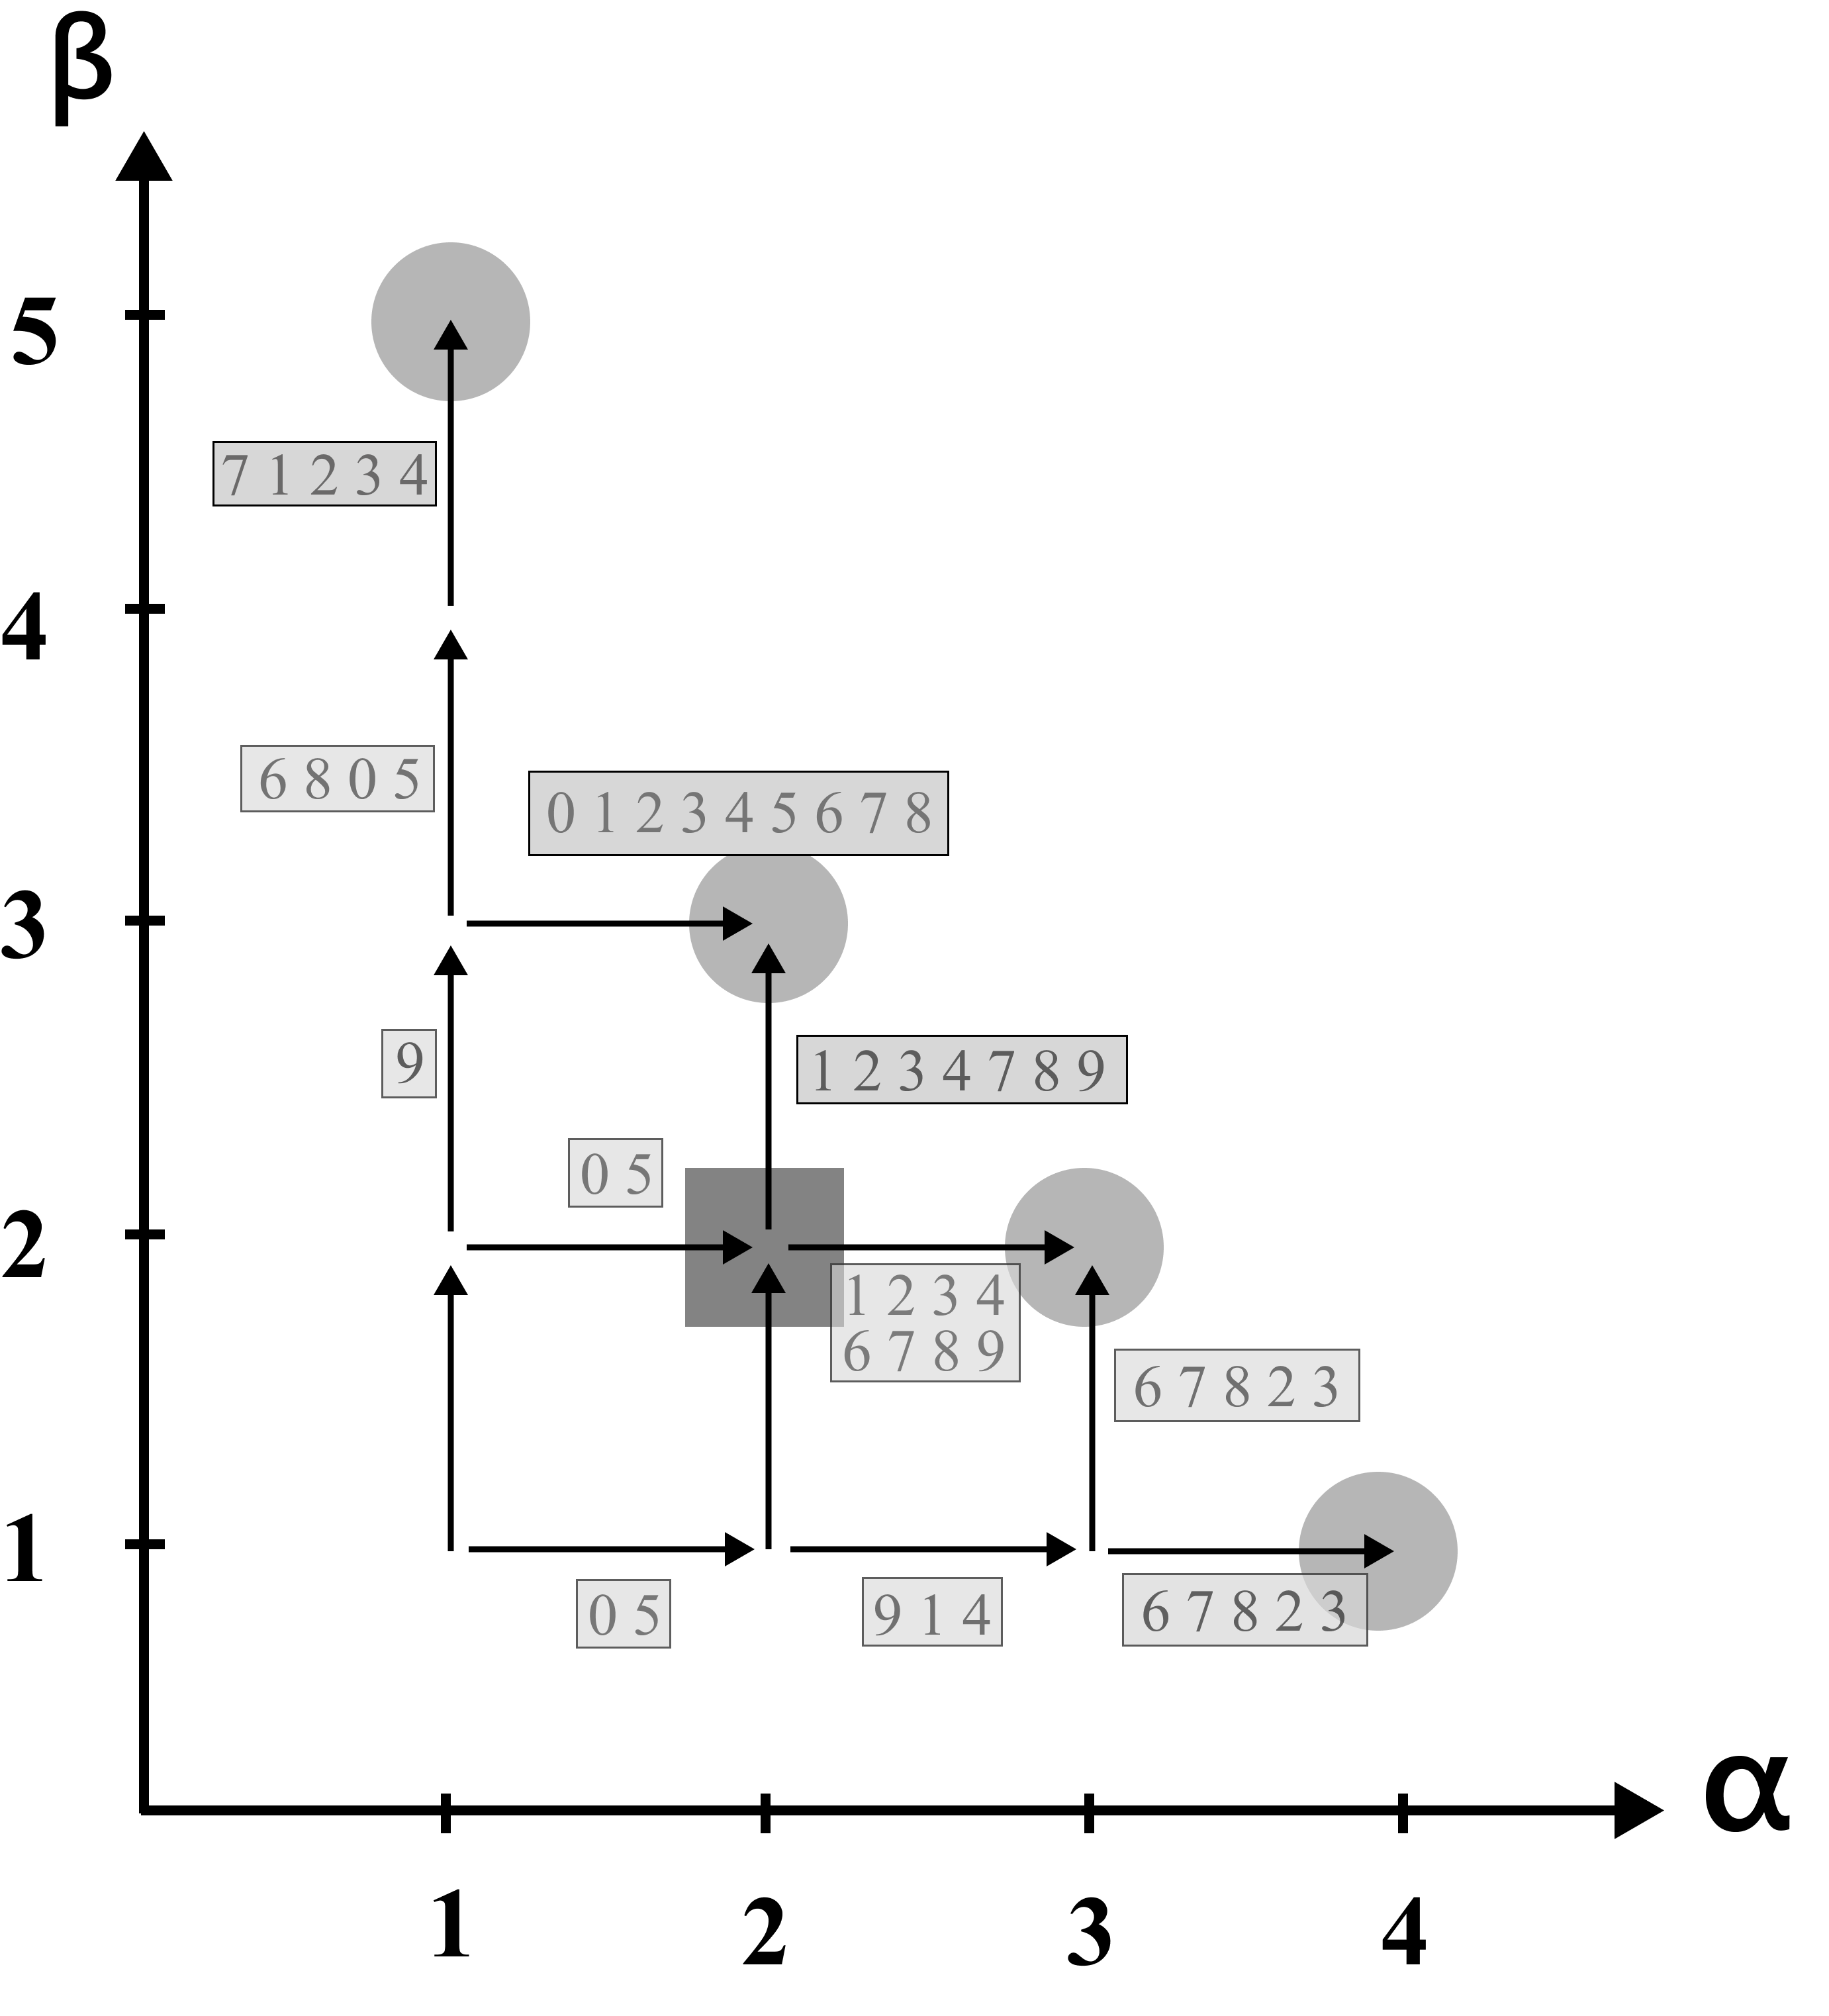
\includegraphics[width=7cm]{figures/diagram1.png} }}%
    \caption{On the left is an example bipartite graph, and on the right is an illustration of the peeling space of the graph. This is discussed in more detail in Section \ref{sec:optim}}%
    \label{fig:peel}%
\end{figure}

\begin{figure}%
    \centering
    \subfloat[\centering Algorithm \ref{alg-par}'s Peeling Path]{{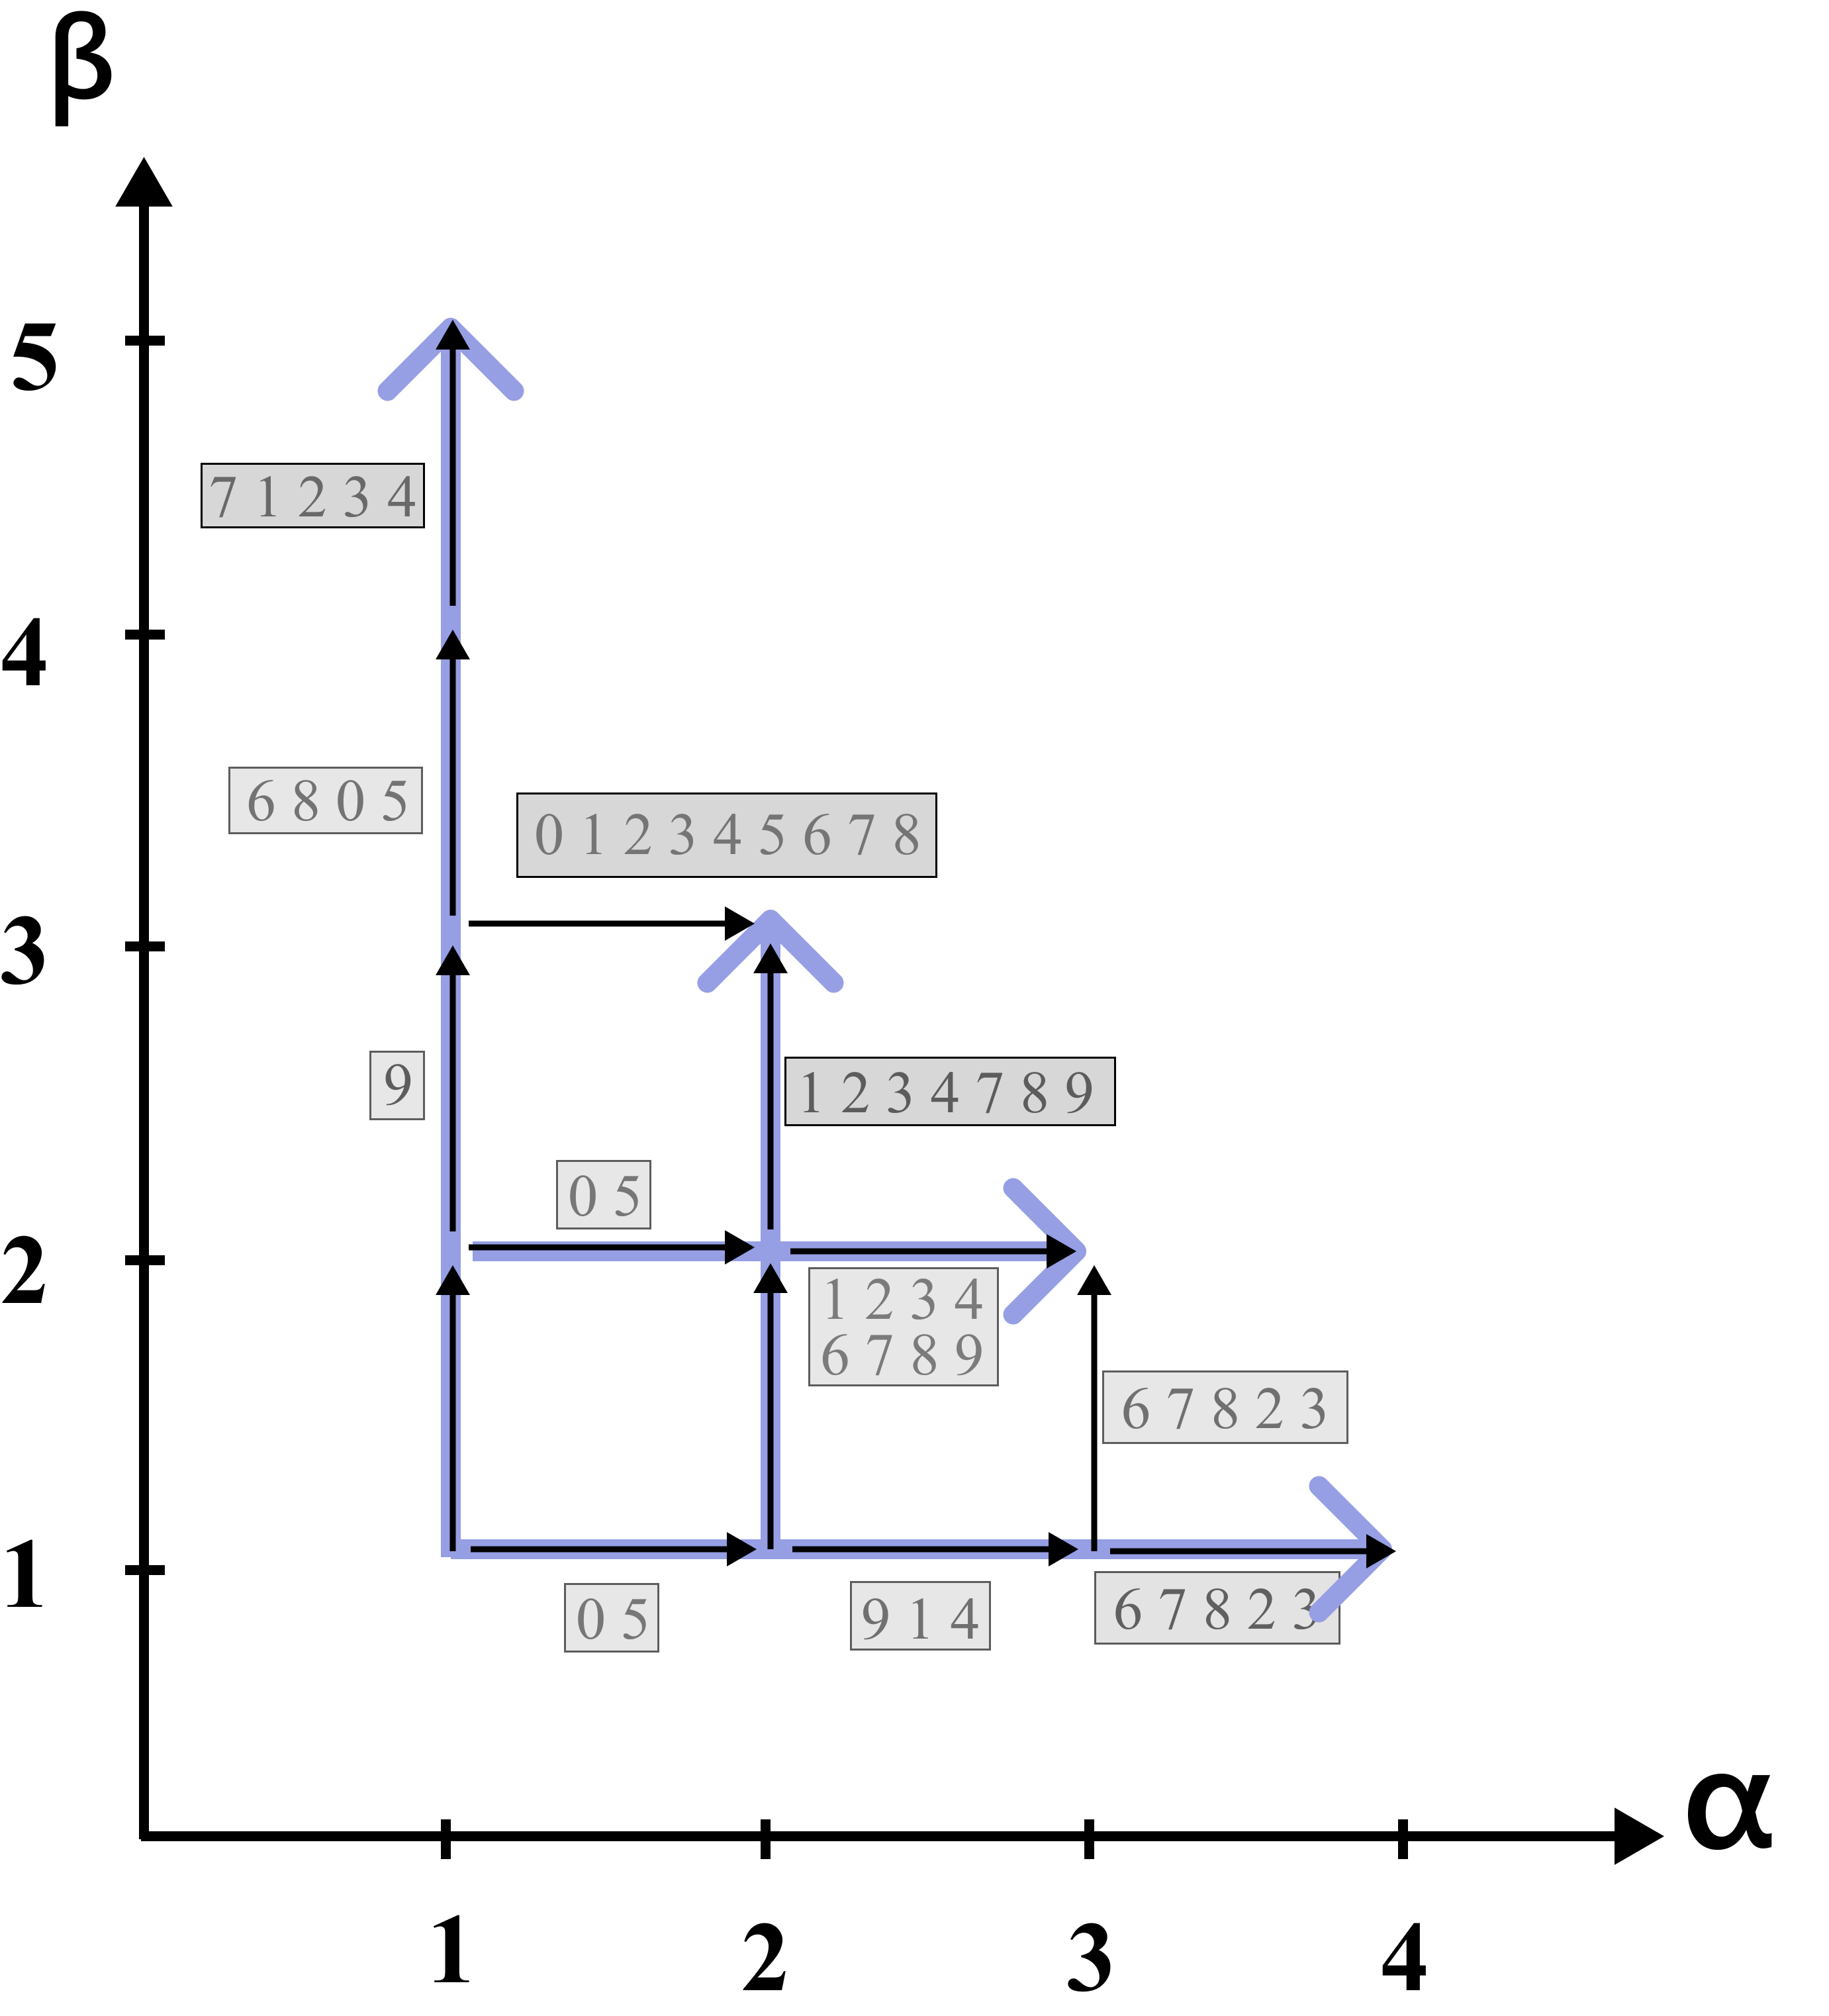
\includegraphics[width=7cm]{figures/diagram2.png} }}%
    \qquad
    \subfloat[\centering Optimized Peeling Path ]{{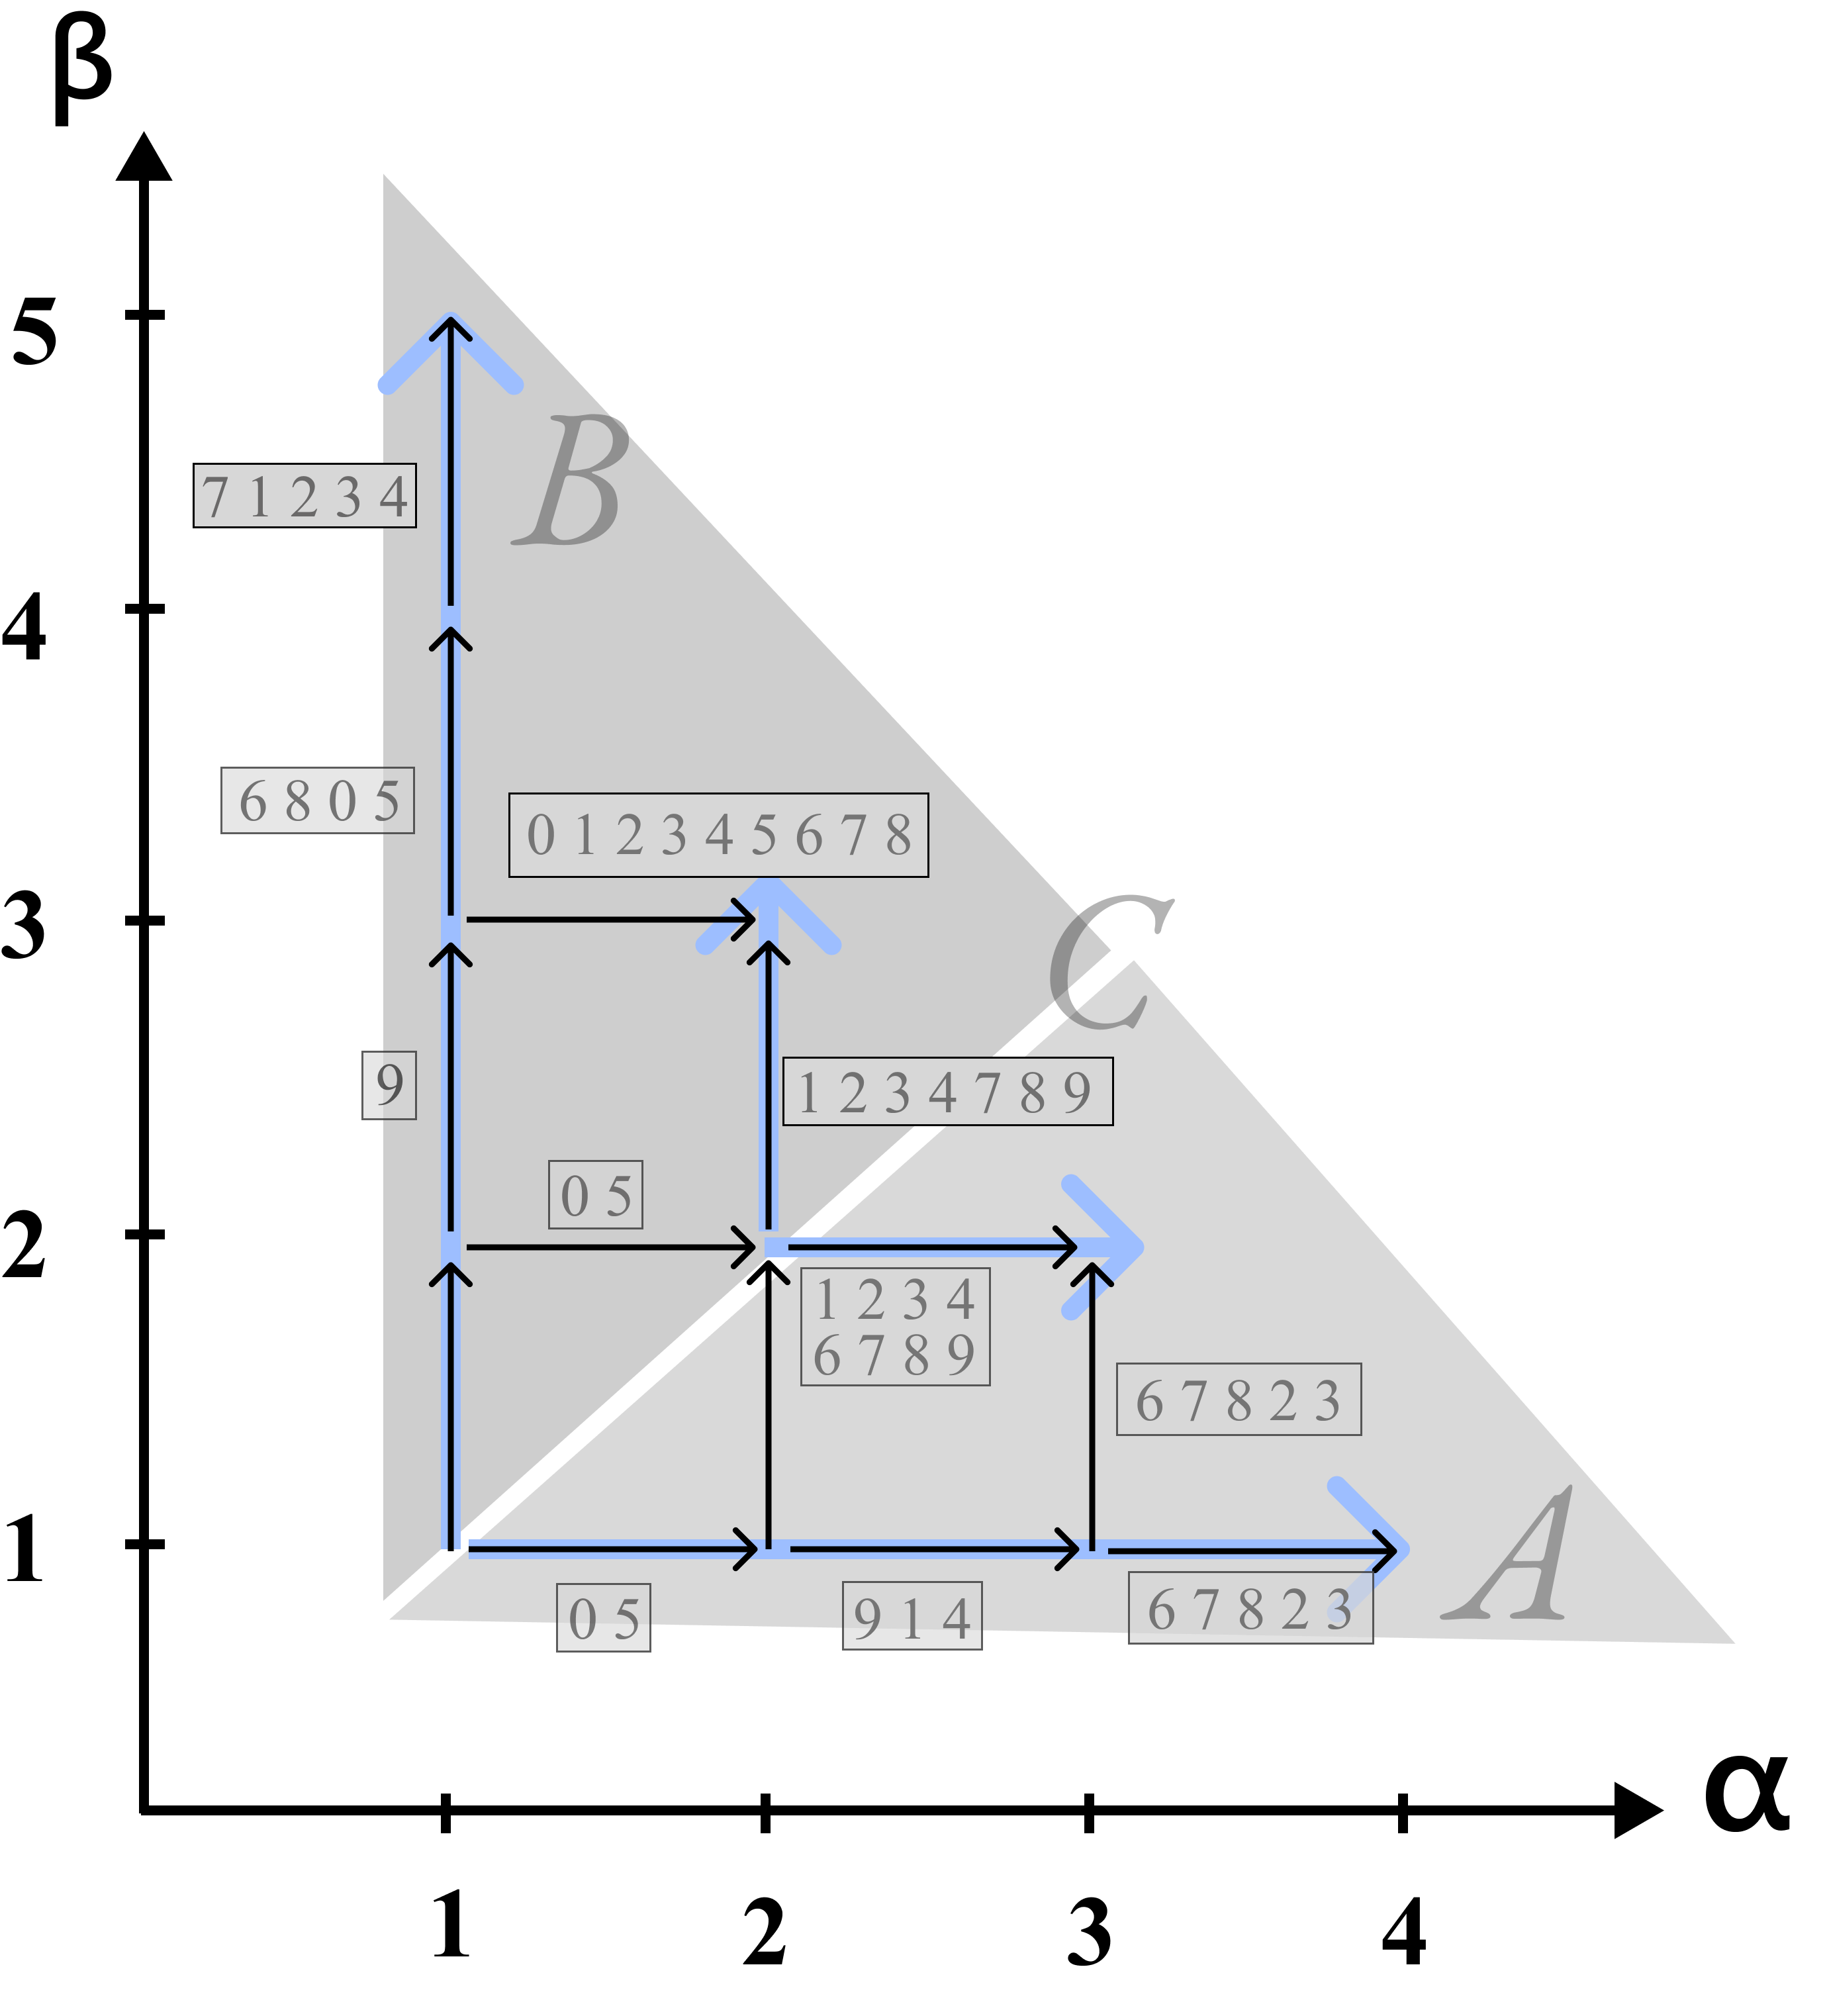
\includegraphics[width=7cm]{figures/diagram3.png} }}%
    \caption{This figure compares unoptimized vs optimized peeling paths. The left hand side shows the unoptimized peeling paths while the right hand side shows the optimized ones.}%
    \label{fig:peelspace}%
\end{figure}

Each integral intersection in the grid of Figure \ref{fig:peel} represents an $(\alpha,\beta)$-core. Edges represent a single-step peeling operation from $(\alpha,\beta)$-core to $(\alpha,\beta+1)$-core (upward) or to $(\alpha+1,\beta)$-core (rightward). The numerals on an edge represents the indices of vertices that would be deleted by that specific peeling operation. The circled nodes represent $(\alpha,\beta)$-cores that are empty, and the boxed node represents the $(\delta,\delta)$-core. Every core corresponding to a grid position that is not drawn is empty. The circled nodes form the boundary of the peeling space.

The peeling operations performed by Algorithm \ref{alg-par} can be visualized by the blue highlighted peeling paths in Figure \ref{fig:peelspace} (a). For $\alpha'=1$, we perform $\beta$-core peeling from $\beta=1$ to $\beta=5$. For $\alpha'=2$, we again increase $\beta$ from $1$ to $3$ while iteratively removing vertices not within the current bi-core. With the proposed optimization, for $\alpha'=2$, we only perform peeling from $\beta=2$ to $\beta=5$, starting from the $(\alpha',\alpha')$-core, or the $(2,2)$-core in this case. This is represented by the blue highlighted peeling paths in Figure \ref{fig:peelspace} (b).

To show the correctness of the optimized algorithm, we divide the peeling space into $3$ parts: part C with the diagonal $(x,x)$-cores, part B where all the $(\alpha,\beta)$-cores satisfy $\beta>\alpha$ and part A where the $(\alpha,\beta)$-cores satisfy $\alpha>\beta$. Note that part A of the peeling space corresponds visually to the part of peeling space below the diagonal $(x,x)$-cores; part B corresponds instead to the section above the diagonal $(x,x)$-cores. Thus, for the optimized algorithm, when peeling along increasing $\alpha$ values, it operates in part A of the peeling space; when peeling along increasing $\beta$ values it operates in part B of the peeling space. 

First, we note that the correct $\alpha_{\max \beta}(v)$ values are computed for all vertices $v$ with $(\alpha_{\max \beta}(v), \beta)$-cores in part A or C of the peeling space. For a specific $\beta$ value, if vertex $v\in (\alpha,\beta)$-core but $v\not\in (\alpha+1,\beta)$-core, with $\alpha\ge \beta$, then $\alpha_{\max \beta}(v)$ is recorded correctly to be $\alpha$ as we perform peeling along $\alpha$ values from $\alpha = \beta$ to its maximum value. 

Then, we show that the optimized algorithm computes the correct $\alpha_{\max \beta}(v)$ values for all vertices $v$ with $(\alpha_{\max \beta}(v), \beta)$-cores in part B of the peeling space. When peeling along increasing $\beta$ values with $\alpha' = \alpha_{\max \beta}(v)$, the algorithm would remove $v$ at $(\alpha_{\max \beta}(v), \beta')$-core, where $\beta'$ is some core value higher than $\beta$.
Given that, the updates of $\alpha_{\max \beta}(v)$ in \algname{par-peel-fix-$\alpha$} in Algorithm \ref{alg-par} as described in Section \ref{sec:par-decomp} ensures the $\alpha_{\max \beta}(v)$ value recorded is $\alpha'$, the correct value. Because A, B, and C form the entire peeling space, we have shown that for all $\beta$ and $v$ values, $\alpha_{\max\beta}(v)$ is correctly recorded. 

Symmetric correctness arguments can be established for $\beta_{\max \alpha}(u)$ values to show that the overall optimized algorithm is correct. 

